\documentclass[article]{IEEEtran}
\usepackage[a5paper, margin=10mm, onecolumn]{geometry}

\usepackage{tfrupee} 
\setlength{\headheight}{1cm} 
\setlength{\headsep}{0mm}       
\usepackage{multicol}
\usepackage{gvv-book}
\usepackage{gvv}
\usepackage{cite}
\usepackage{amsmath,amssymb,amsfonts,amsthm}
\usepackage{algorithmic}
\usepackage{graphicx}
\usepackage{textcomp}
\usepackage{xcolor}
\usepackage{txfonts}
\usepackage{listings}
\usepackage{enumitem}
\usepackage{mathtools}
\usepackage{gensymb}
\usepackage{comment}
\usepackage[breaklinks=true]{hyperref}
\usepackage{tkz-euclide} 
\usepackage{listings}

\def\inputGnumericTable{}                                 
\usepackage[latin1]{inputenc}                                
\usepackage{color}                       

\usepackage{array}                                            
\usepackage{longtable}                                   

\usepackage{calc}                                             
\usepackage{multirow}                                         
\usepackage{hhline}          

\usepackage{ifthen}                                           
\usepackage{lscape}
\begin{document}
	\title{10.6.8}
	\author{EE25BTECH11052 - Shriyansh Kalpesh Chawda}
	\maketitle
	\textbf{Question}\\
	Construct a pair of tangents to a circle of radius 4cm from a point P lying outside the circle at 
	a distance of 6cm from the centre.
	\hfill{(10, 2023)}\\
	
	\textbf{Solution}\\
	Let the center of the circle be at origin and point P be at distance 6 from center along x-axis.
	\begin{align}
		O &= \myvec{0\\0}\\
		P &= \myvec{6\\0}
	\end{align}
	The equation of the circle $x^2 + y^2 = 16$ can be written as:
	\begin{align}
		\vec{x}^\top \vec{x} - 16 &= 0
	\end{align}
	The parameters of the circle are:
	\begin{equation}
		\vec{V} = \vec{I}, \quad \vec{u} = \vec{0}, \quad f = -16
	\end{equation}
	
	Let the point of contact be $\vec{q}$ and
	\begin{align}
		\vec{q}^\top\vec{q} = 16
	\end{align}
	
	From the condition of tangency we get:
	\begin{align}
		\vec{q}^\top(\vec{q} - P) &= 0\\
		P^\top\vec{q} &= \vec{q}^\top\vec{q}\\
		P^\top\vec{q} &= 16
	\end{align}
	
	Let the tangent equation passing through $P$ be:
	\begin{align}
		\vec{x} = P + k\vec{m}
	\end{align}
	where $\vec{m}$ is the direction vector of the tangent.
	
	Substituting into the circle equation:
	\begin{align}
		g(\vec{x}) &= \vec{x}^\top\vec{x} - 16\\
		(P + k\vec{m})^\top(P + k\vec{m}) - 16 &= 0\\
		k^2\vec{m}^\top\vec{m} + 2kP^\top\vec{m} + P^\top P - 16 &= 0\\
		k^2\vec{m}^\top\vec{m} + 2kP^\top\vec{m} + g(P) &= 0
	\end{align}
	
	As the tangent intersects the conic at only one point (the point of contact), the discriminant for the quadratic in $k$ is equal to 0:
	\begin{align}
		4(P^\top\vec{m})^2 - 4\vec{m}^\top\vec{m} \cdot g(P) &= 0\\
		(P^\top\vec{m})^2 - g(P)\vec{m}^\top\vec{m} &= 0
	\end{align}
	
	Since $P = \myvec{6\\0}$:
	\begin{align}
		g(P) = P^\top P - 16 = 36 - 16 = 20
	\end{align}
	
	The discriminant condition becomes:
	\begin{align}
		\vec{m}^\top Q\vec{m} = 0
	\end{align}
	where
	\begin{align}
		Q = \myvec{-(P^\top P) & 0\\0 & g(P)} = \myvec{-36 & 0\\0 & 20}
	\end{align}
	
	\textbf{Eigenvalue Decomposition of Q:}\\
	As $Q$ is a diagonal matrix, the eigenvalues are the diagonal entries:
	\begin{equation}
		\lambda_1 = -36, \quad \lambda_2 = 20
	\end{equation}
	
	Applying eigenvalue decomposition for $Q$:
	\begin{align}
		Q = XDX^\top
	\end{align}
	where
	\begin{align}
		D = \myvec{-36 & 0\\0 & 20}
	\end{align}
	
	$X$ is an orthogonal matrix whose columns are the corresponding normalized eigenvectors of $Q$. As $Q$ is a diagonal matrix:
	\begin{equation}
		X = \vec{I}
	\end{equation}
	
	From $\vec{m}^\top Q\vec{m} = 0$:
	\begin{align}
		\vec{m}^\top XDX^\top\vec{m} &= 0
	\end{align}
	
	Let $\vec{z} = X^\top\vec{m}$. Then:
	\begin{align}
		\vec{z}^\top D\vec{z} &= 0\\
		\myvec{z_1 & z_2}\myvec{-36 & 0\\0 & 20}\myvec{z_1\\z_2} &= 0\\
		-36z_1^2 + 20z_2^2 &= 0\\
		\frac{z_1^2}{z_2^2} &= \frac{20}{36} = \frac{5}{9}\\
		\frac{z_1}{z_2} &= \pm\frac{\sqrt{5}}{3}
	\end{align}
	
	Solving for $\vec{m}$:
	\begin{align}
		\vec{I}\vec{m} &= \vec{z}\\
		\vec{m} &= \myvec{z_1\\z_2}
	\end{align}
	
	From $z_1/z_2 = \pm\sqrt{5}/3$, the direction vectors for the tangents can be expressed as:
	\begin{align}
		\vec{m}_1 = \myvec{\sqrt{5}\\3}, \quad \vec{m}_2 = \myvec{\sqrt{5}\\-3}
	\end{align}
	
	\textbf{Finding Points of Contact:}\\
	Using $P^\top\vec{q} = 16$:
	\begin{align}
		\myvec{6 & 0}\myvec{q_1\\q_2} &= 16\\
		6q_1 &= 16\\
		q_1 &= \frac{8}{3}
	\end{align}
	
	From $q_1^2 + q_2^2 = 16$:
	\begin{align}
		\brak{\frac{8}{3}}^2 + q_2^2 &= 16\\
		q_2^2 &= 16 - \frac{64}{9} = \frac{80}{9}\\
		q_2 &= \pm\frac{4\sqrt{5}}{3}
	\end{align}
	
	Therefore, the points of contact are:
	\begin{align}
		\vec{q}_1 = \myvec{\frac{8}{3}\\\frac{4\sqrt{5}}{3}}, \quad \vec{q}_2 = \myvec{\frac{8}{3}\\-\frac{4\sqrt{5}}{3}}
	\end{align}
	
	\textbf{Equations of Tangents:}\\
	The tangent at $\vec{q}$ is given by: $\vec{q}^\top\vec{x} = 16$.\\
	\textbf{Tangent 1} at $\vec{q}_1$:
	\begin{align}
		\myvec{\frac{8}{3} & \frac{4\sqrt{5}}{3}}\myvec{x\\y} &= 16\\
		\frac{8}{3}x + \frac{4\sqrt{5}}{3}y &= 16\\
		2x + \sqrt{5}y &= 12
	\end{align}	
	\textbf{Tangent 2} at $\vec{q}_2$:
	\begin{align}
		\myvec{\frac{8}{3} & -\frac{4\sqrt{5}}{3}}\myvec{x\\y} &= 16\\
		2x - \sqrt{5}y &= 12
	\end{align}
	The equations of the pair of tangents are:
	\begin{align}
		\boxed{2x + \sqrt{5}y = 12 \quad \text{and} \quad 2x - \sqrt{5}y = 12}
	\end{align}
	
	\begin{figure}[H]
		\centering
		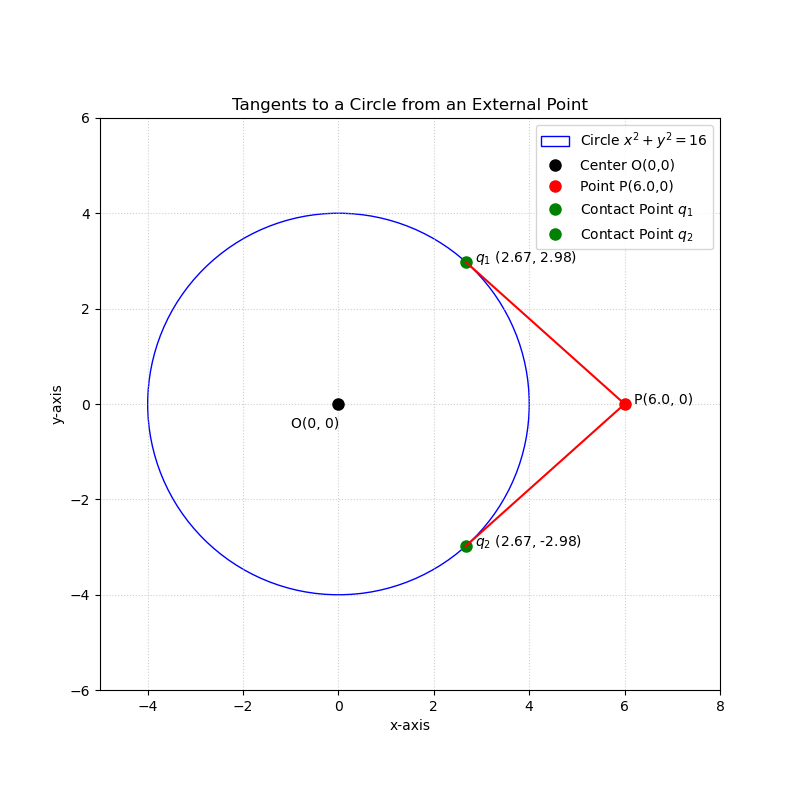
\includegraphics[width=1.1\linewidth]{figs/tangents_plot}
	\end{figure}
	
\end{document}